% set PDF output version to 1.7
\pdfminorversion=7

\documentclass[
fontsize=12pt,          % Schriftgroesse
paper=a4,               % Papiergroesse
captions=tableabove,    % Beschriftungen fuer Tabellen oberhalb
titlepage=firstiscover, % Titelseite ist Umschlagseite
BCOR=5mm,               % Korrektur fuer Bundsteg
toc=listof,             % Abbildungs- und Tabellenverzeichnis im Inhaltsverzeichnis
open=right,             % Kapitel beginnen auf rechter Seite
]{scrreprt}

\KOMAoptions{DIV=12}

% ----------------------------------------------------
% Essential packages
% ----------------------------------------------------
\usepackage[utf8]{inputenc}
\usepackage[T1]{fontenc}

% ----------------------------------------------------
% Packages for layout adjustments
% ----------------------------------------------------

% Adjust line spacing
\usepackage{setspace}

% Publication quality tables
\usepackage{booktabs}

% ----------------------------------------------------
% Fonts
% ----------------------------------------------------
\usepackage{lmodern}
\usepackage{fix-cm}
\rmfamily
\DeclareFontShape{T1}{lmr}{b}{sc}{<->ssub*cmr/bx/sc}{}
\DeclareFontShape{T1}{lmr}{bx}{sc}{<->ssub*cmr/bx/sc}{}
\usepackage{roboto}

\setkomafont{subject}{\large}
\setkomafont{title}{\LARGE\bfseries} % \robotocondensed yields font warning
\setkomafont{subtitle}{\Large} % \robotocondensed yields font warning
\setkomafont{author}{\Large}
\setkomafont{date}{\small}
%\addtokomafont{publishers}{\normalsize\robotocondensed}

% ----------------------------------------------------
% Colors
% ----------------------------------------------------
\usepackage{graphicx}
\usepackage[svgnames]{xcolor}
\definecolor{darkgreen}{rgb}{0.23,0.46,0.23}
\definecolor{smdsblue}{RGB}{0,69,134}

% ----------------------------------------------------
% Internal commands
% ----------------------------------------------------

\usepackage{etoolbox}
\makeatletter
\newcommand{\degree}[1]{\gdef\@degree{#1}}
\newcommand{\course}[1]{\gdef\@course{#1}}
\newcommand{\email}[1]{\gdef\@email{#1}}
\newcommand{\matrno}[1]{\gdef\@matrno{#1}}
\newcommand{\institute}[1]{\gdef\@institute{#1}}
\newcommand{\director}[4]{%
  \gdef\@director@name{#1}%
  \gdef\@director@title{#2}%
  \gdef\@director@firstaffiliation{#3}%
  \gdef\@director@secondaffiliation{#4}%
}
\newcommand{\coordinator}[4]{%
  \gdef\@coordinator@name{#1}%
  \gdef\@coordinator@title{#2}%
  \gdef\@coordinator@firstaffiliation{#3}%
  \gdef\@coordinator@secondaffiliation{#4}%
}
\newcommand{\organization}[3]{%
  \gdef\@organization@name{#1}%
  \gdef\@organization@address{#2}%
  \gdef\@organization@city{#3}%
}
\makeatother

% Sprachauswahl:
%  main=* setzt die Hauptsprache fuer das Dokument
%  - ngerman --> deutsch
%  - english --> englisch
%\def\languages{main=ngerman,english}
\def\languages{main=american,british,french}

% Art der Arbeit (= Bachelorarbeit, Masterarbeit)
\subject{Internship report}

% Studiengang und angestrebter Abschluss
\course{Computer Science INF591}
\degree{Master 1 - Jacques Herbrand}

% Haupt- und (optional) Untertitel der Arbeit
\title{Stack Buffer Overflows}
\subtitle{Attacks and defense mechanisms}

% Name, Matrikelnummer und E-Mail-Adresse
\author{Florian \textsc{Hofhammer}}
\matrno{XXXXXXXX}
\email{florian.hofhammer@polytechnique.edu}

% Datum der Abgabe
\date{07/07/2020}

% Internship dates
\gdef\dates{01/04/2020 - 30/06/2020}

% Affiliations
\gdef\DIX{Computer Science Departement, École Polytechnique}
\gdef\FLARE{FLaRe, Facebook Research}
\gdef\INRIA{Inria Sophia Antipolis - Méditerranée}
\gdef\DIUC{I3S, Université Côte d'Azur}

% Host organization
\organization{\DIUC}{2000, route des Lucioles}{06900 Sophia Antipolis}

% Academic and host organization supervisors and their affiliations
\coordinator{Francesco \textsc{Zappa Nardelli}}{Professor}{\FLARE}{\DIX}
\director{Sid \textsc{Touati}}{Professor}{\INRIA}{\DIUC}

%%% Optionen fuer den Druck:
\KOMAoption{twoside}{no}  % Einseitiger Druck
%\KOMAoption{twoside}{yes}   % Doppelseitiger Druck (Duplex)

% Entwurfsmodus: Mehr Warnungen (z.B. bei zu vollen Zeilen)
\KOMAoption{draft}{yes}

%%% Local Variables:
%%% mode: latex
%%% TeX-master: "Report"
%%% End:


% ----------------------------------------------------
% Multi-lingual documents with Babel
% ----------------------------------------------------
\usepackage{csquotes}
\usepackage[\languages]{babel}

% ----------------------------------------------------
% Hyperlinks in PDF documents
% ----------------------------------------------------
\usepackage[%
bookmarks=true,         %
bookmarksopenlevel=1,   %
bookmarksopen=true,     %
bookmarksnumbered=true, %
plainpages=false,       % correct hyperlinks
pdfpagelabels=true,     % view TeX pagenumber in PDF reader
colorlinks=true,        % color highlight links
allcolors=black,        % make all links black by default
urlcolor=smdsblue,      % URL color
]{hyperref}

\makeatletter
\AtEndPreamble{
  \hypersetup{
    pdftitle=\@title,
    pdfauthor=\@author
  }
}
\makeatother

% Provides a solution to the problem with hyperref that links
% to floats actually anchor to the place below the float's caption,
% instead of anchoring to the beginning of the float
\usepackage[all]{hypcap}

% ----------------------------------------------------
% Code listings
% ----------------------------------------------------
\definecolor{commentgreen}{rgb}{0,0.6,0}
\definecolor{stringmauve}{rgb}{0.58,0,0.82}

\usepackage{listings}
\renewcommand*{\lstlistlistingname}{List of Listings}
\lstset{%
  frame=single,                             % Add a single line frame around listings
  breaklines=true,							% Automatic line breaks
  backgroundcolor=\color{gray!3},           % Slight gray shade for listings
  rulecolor=\color{black!30},               % Gray frame outline
  xleftmargin=.1\textwidth,                 % Extra left margin
  xrightmargin=.1\textwidth,                % Extra right margin
  basicstyle=\footnotesize\ttfamily,        % General font style for listings
  keywordstyle=\bfseries\color{blue},       % Font style for keywords
  commentstyle=\color{commentgreen},        % Font style for comments
  stringstyle=\color{stringmauve},          % Font style for string literals
  numbers=left,                             % Show line numbers
  stepnumber=1,                             % Step increments for line numbers
  numberstyle={\sffamily\tiny\color{gray}}, % Font style for line numbers
  numbersep=2em,                            % Space between line numbers and code
%  captionpos=b,								% Caption below listing
}


% ----------------------------------------------------
% Bibliography management
% ----------------------------------------------------
\usepackage[%
backend=biber,      % Use biber to process bibliographies
natbib=true,        % Provide natbib-compatible citation commands
%sorting=none,       % Sort citations by occurrence in the document
sorting=nty,		% Sort after name, title, year
style=numeric-comp, % Use compressed numeric citations, e.g. [1-3; 5]
block=space,        % Add a little spacing inside bibliography entries
]{biblatex}
\addbibresource{literature.bib}

% Use main body font for URLs in bibliography
\urlstyle{same}

% Allow linebreaks in URLs to prevent really ugly overfull hboxes
\setcounter{biburllcpenalty}{7000}
\setcounter{biburlucpenalty}{8000}


% ----------------------------------------------------
% Localization / translations
% ----------------------------------------------------
\usepackage{translations}

% Generic translation used in template
\NewTranslation{ngerman}{coordinator}{Praktikumskoordinator}
\NewTranslation{ngerman}{director}{Praktikumsbetreuer}
\NewTranslation{ngerman}{matrno}{Matrikelnummer}
\NewTranslation{ngerman}{institute}{Computer Science Department\\École Polytechnique}
\NewTranslation{ngerman}{hostorga}{Host-Organisation}
\NewTranslation{ngerman}{duedate}{Abgabedatum}
\NewTranslation{ngerman}{dates}{Daten}
\NewTranslation{ngerman}{regularlit}{Literatur}
\NewTranslation{ngerman}{onlinelit}{Online-Quellen}
\NewTranslation{ngerman}{honesty@title}{Eidesstattliche Erkl\"{a}rung}
\NewTranslation{ngerman}{honesty@body}{%
  Ich versichere, dass ich die vorliegende Arbeit ohne fremde Hilfe und ohne Benutzung anderer
  als der angegebenen Quellen angefertigt habe, und dass die Arbeit in gleicher oder \"{a}hnlicher
  Form noch keiner anderen Pr\"{u}fungsbeh\"{o}rde vorgelegen hat.\endgraf
  Alle Ausf\"{u}hrungen der Arbeit, die w\"{o}rtlich oder sinngem\"{a}\ss{} \"{u}bernommen wurden, sind als solche
  gekennzeichnet.
}

% English fallback text
\NewTranslationFallback{coordinator}{Internship coordinator}
\NewTranslationFallback{director}{Internship director}
\NewTranslationFallback{matrno}{Matriculation number}
\NewTranslationFallback{institute}{Computer Science Department\\École Polytechnique}
\NewTranslationFallback{hostorga}{Host organization}
\NewTranslationFallback{duedate}{Submission date}
\NewTranslationFallback{dates}{Dates}
\NewTranslationFallback{regularlit}{Literature}
\NewTranslationFallback{onlinelit}{Online resources}
\NewTranslationFallback{honesty@title}{Declaration of Academic Honesty}
\NewTranslationFallback{honesty@body}{%
  Hereby, I declare that I have composed the presented paper independently on my own and without
  any other resources than the ones indicated. All thoughts taken directly or indirectly from external
  sources are properly denoted as such.\endgraf
  This paper has neither been previously submitted to another authority nor has it been published yet.
}


% ----------------------------------------------------
% Additional packages and configuration
% ----------------------------------------------------

% Landscape pages
%\usepackage{lscape}

% Resolve float warnings referring to the ToC
\usepackage{tocbasic}
\usepackage{scrhack}

% Bibliography numbering independent of ToC and lists (of figures, tables, listings)
\usepackage{notoccite}

% Subfigures
\usepackage{caption}
\usepackage{subcaption}

% Improvements to math mode
\usepackage{amsmath}
\usepackage{amssymb}

% Table improvements
%\usepackage{longtable} % not in use right now
%\usepackage{multirow}
\usepackage{array}
\newcolumntype{P}[1]{>{\centering\arraybackslash}m{#1}} % Centered column with fixed width
\newcommand{\tabitem}{{\textbullet}~}
\newcommand{\rotatecell}[1]{\begin{tabular}{@{}c@{}}\rotatebox[origin=c]{90}{#1}\end{tabular}}

% todonotes: Adds todo notes
\setlength{\marginparwidth}{2cm}
\usepackage[english]{todonotes}

% glossaries: Adds possibility to create a glossary
\usepackage[toc, automake, acronyms, nomain, shortcuts]{glossaries}
\makeglossaries
\GlsSetQuote{+}

% Footnote enhancements
% Don't reset footnote numbering for every chapter
\counterwithout{footnote}{chapter}
% Don't split footnote over several pages
\interfootnotelinepenalty=10000 

% Enable emergency line breaks to prevent over-full boxes
\emergencystretch=1em

% Suppress PDF group warning, has no bad effect
\pdfsuppresswarningpagegroup=1

% Checkmark and crossmark
\usepackage{pifont}
\newcommand{\cmark}{\ding{51}}
\newcommand{\xmark}{\ding{55}}

% Additional cross referencing tools, like e.g. lowercase nameref
\usepackage{crossreftools}

% Intelligent cross-referencing
% Note: Must be loaded at end of preamble (esp. after hyperref)
\usepackage[nameinlink,noabbrev]{cleveref}

%%% Local Variables:
%%% mode: latex
%%% TeX-master: "Report"
%%% End:


\newacronym{ascii}{ASCII}{American Standard Code for Information Interchange}
\newacronym{aslr}{ASLR}{Address Space Layout Randomization}
\newacronym{cet}{CET}{Control-flow Enforcement Technology}
\newacronym{cfi}{CFI}{Control Flow Integrity}
\newacronym{cop}{COP}{Call-oriented Programming}
\newacronym{dep}{DEP}{Data Execution Prevention}
\newacronym{elf}{ELF}{Executable and Linking Format}
\newacronym{gcc}{GCC}{GNU Compiler Collection}
\newacronym{glibc}{glibc}{GNU C Library}
\newacronym{gnu}{GNU}{GNU's Not Unix}
\newacronym{got}{GOT}{Global Offset Table}
\newacronym{jit}{JIT}{just-in-time}
\newacronym{jop}{JOP}{Jump-oriented Programming}
\newacronym{lifo}{LIFO}{last in, first out}
\newacronym{lts}{LTS}{Long-term support}
\newacronym{nop}{NOP}{no operation}
\newacronym{nx}{NX}{no-execute}
\newacronym{pae}{PAE}{Physical Address Extension}
\newacronym{pic}{PIC}{Position Independent Code}
\newacronym{pie}{PIE}{Position Independent Executable}
\newacronym{plt}{PLT}{Procedure Linkage Table}
\newacronym{relro}{RELRO}{Relocation Read-Only}
\newacronym{ret2libc}{ret2libc}{return-to-libc}
\newacronym{rip}{RIP}{Return Instruction Pointer}
\newacronym{rop}{ROP}{Return-oriented Programming}
\newacronym{sfp}{SFP}{Saved Frame Pointer}
\newacronym{ssp}{SSP}{Stack Smashing Protectors}
\newacronym{stdin}{stdin}{standard input}
\newacronym[plural={opcodes}, firstplural={operation codes / instruction codes}]{opcode}{opcode}{operation code / instruction code}
\newacronym[plural={OSs}]{os}{OS}{Operating System}
\newacronym{wxorx}{W$ \oplus $X}{write-xor-execute}
\newacronym{xd}{XD}{execute-disable}
\makeglossaries

\begin{document}
% Titelei
%% Cover/title page
\begin{titlepage}
  \onehalfspacing
  \makeatletter
  \vspace*{1em}
  \begin{center}
    {\LARGE\textsc{École Polytechnique}}\\[0.2em]
    {\Large Institut Polytechnique de Paris}

    \par\vspace{3em}
    {\usekomafont{subject}%
      \@subject\\
      for the \@course \space internship\par
      in the \@degree \space program
    }\\

    {\usekomafont{date}
	  \dates
    }\\

    \vfill
    {\usekomafont{title}\@title}
    \ifdefempty{\@subtitle}{}{%
      \par\vspace{.5em}
      {\usekomafont{subtitle}\@subtitle}
    }
    
    \par\vspace{2em}
    {\usekomafont{author}\@author}
  \end{center}
  \makeatother

  \vfill
  \centering
  
\includegraphics[height=100mm]{figures/Ecole_polytechnique_signature}\\
  
\includegraphics[width=.3\paperwidth]{figures/inr_logo_rouge_rvb}
  \hspace*{2em}
  
\includegraphics[width=.3\paperwidth]{figures/NewlogoI3S}\\[-5em]
\end{titlepage}

%% \GetTranslation{matrno}: \@matrno\par

%% Credits
\makeatletter
\clearpage
\thispagestyle{empty}
\vspace*{\fill}
\noindent\@author\\[0.2em]
\noindent\textbf{\@title}

\begin{tabbing}
  This is just a placeholder \= Here comes the content \kill
  \GetTranslationFor{american}{coordinator}: \> \textbf{\@coordinator@name}, \@coordinator@title \\
  \> \@coordinator@firstaffiliation\\
  \> \@coordinator@secondaffiliation\\[2mm]
  \GetTranslationFor{american}{director}: \> \textbf{\@director@name}, \@director@title \\
  \> \@director@firstaffiliation\\
  \> \@director@secondaffiliation\\[2mm]
  \GetTranslationFor{american}{hostorga}: \> \@organization@name \\
  \> \@organization@address \\
  \> \@organization@city \\[2mm]
%  \GetTranslationFor{american}{matrno}: \> \@matrno\\[2mm]
%  \GetTranslationFor{american}{duedate}: \> \@date
  \GetTranslationFor{american}{dates}: \> \dates
\end{tabbing}
\vspace*{-5em}
\makeatother

%%% Local Variables:
%%% mode: latex
%%% TeX-master: "Report"
%%% End:

\pdfbookmark[1]{\abstractname}{abstract}
\newenvironment{abstractpage}
  {\cleardoublepage\thispagestyle{empty}\chapter*{\abstractname}}
  {\cleardoublepage}
\renewenvironment{abstract}[1]
  {\bigskip\begin{otherlanguage}{#1}%
   \begin{center}\bfseries\abstractname\end{center}\noindent}
  {\end{otherlanguage}\par\bigskip}

\begin{abstractpage}
  \begin{abstract}{american}
    The goal of the presented paper is to summarize different stack buffer overflow attack and defense methods in a single paper.
    In this context, the question arises how some defense methods can be bypassed by an attacker and how a defender can improve on the defense mechanisms to thwart stack buffer overflow based attacks.

    To achieve these goals and answer these questions, several attack methods and their implications on the security of currently deployed defense mechanisms are presented.
    They show that even on modern systems, stack buffer overflow vulnerabilities can be exploited to execute arbitrary code controlled by an attacker under specific circumstances.
    Although stack buffer overflows are hard or impossible to exploit depending on the circumstances of the vulnerability and the system configuration, the need for security measure enhancements arises.
    Such improvements and expansions on current defense mechanisms against stack buffer overflows are also presented and compared with regard to their performance implications on a system.
  \end{abstract}
  \vspace{2em}
  \begin{abstract}{french}
    L'objectif de l'article présenté est de résumer en un seul document les différentes méthodes d'attaque et de défense contre les débordements de pile.
    Dans ce contexte, la question se pose de savoir comment certaines méthodes de défense peuvent être contournées par un attaquant et comment un défenseur peut améliorer les mécanismes de défense pour contrecarrer les attaques basées sur le débordement de pile.

    Pour atteindre ces objectifs et répondre à ces questions, plusieurs méthodes d'attaque et leurs implications sur la sécurité des mécanismes de défense actuellement déployés sont présentées.
    Elles montrent que même sur les systèmes modernes, les vulnérabilités liées au débordement de pile peuvent être exploitées pour exécuter du code arbitraire contrôlé par un attaquant dans des circonstances spécifiques.
    Bien que les débordements de pile soient difficiles ou impossibles à exploiter selon les circonstances de la vulnérabilité et la configuration du système, il est nécessaire d'améliorer les mesures de sécurité.
    Ces améliorations et extensions des mécanismes de défense actuels contre les débordements de pile sont également présentées et comparées en ce qui concerne leurs implications sur les performances d'un système.
  \end{abstract}
\end{abstractpage}

%%% Local Variables:
%%% mode: latex
%%% TeX-master: "Report"
%%% End:

\pdfbookmark[1]{\contentsname}{toc}
\tableofcontents
\listoffigures
\listoftables
\lstlistoflistings
\printglossaries


% Hauptinhalt der Arbeit
\chapter{Introduction}
\label{chp:introduction}

\todo[inline]{Basic introduction here}

\section{Basic vocabulary}
As this report is about stack buffer overflows, it is important to know what this wording means.
The \emph{stack} is a data structure used in modern \gls{os} memory management and is explained in \cref{sec:process-memory,sec:stack-setup-and-usage}.

A \emph{buffer} generally is a ``limited, contiguously allocated set of memory'' \cite[12]{Anley2007}.
In this report, we will often refer to C programming language's \texttt{char} arrays as buffers.
Such arrays are fulfilling the above definition and are generally used to hold \gls{ascii} encoded text or arbitrary binary data, as a \texttt{char} in C refers to exactly one byte of data.

\section{System model}
\label{sec:system-model}

In the cases where references to the Linux kernel, the \gls{glibc} or the \gls{gcc} are made, they refer to specific versions of those software products.
In later versions, the behavior might change in order to mitigate some of the weaknesses described in this report.

Those specific software versions comprise version 5.4.42 of the Linux kernel%
	\footnote{Source code can be viewed online at \href{https://git.kernel.org/stable/h/v5.4.42}{git.kernel.org}}%
.
This release is a \gls{lts} release which means that it will be maintained until the end of 2021 \cite{LKO2020}.
The version of \gls{glibc} is 2.31%
	\footnote{Source code can be viewed online at \href{https://sourceware.org/git/?p=glibc.git;a=tree;h=6ee690ef6fa36bf79d2e05b5a30a4f7e10ba3937;hb=9ea3686266dca3f004ba874745a4087a89682617}{sourceware.org}}%
.
\gls{gcc} is used in in the latest 9.x line version 9.3.0.

At the time of writing this report, newer stable releases of the Linux kernel and \gls{gcc} are already available (5.6.14 for the Linux kernel \cite{LKO2020a}, 10.1 for \gls{gcc} \cite{FSF2020}).
\todo{Look up whether the referenced parts changed at all or if everything's still valid for the new versions}
However, this does not impose any problems on the real-world consequences of this report's contents.
The newest editions of popular Linux distributions for \texttt{x86\_64/amd64} processor architectures like Red Hat Enterprise Linux (version 8.2), Ubuntu (version 20.04 \gls{lts}), Debian (version 10.4) are based on the Linux 5.4.0 \gls{lts} kernel or even older versions%
	\footnote{See also discussion on \href{https://www.reddit.com/r/webhosting/comments/beg0z0/should_i_use_an_lts_version_of_ubuntu_for_my_web/}{reddit.com} on whether to use \gls{lts} versions for production server deployment}
\cite{RedHat2020,Canonical2020,SPI2020,SPI2020a}.
Also, the highest kernel version used for development of the Android mobile \gls{os}, which has a market share of about 70\% \cite{Statcounter2020}, is Linux 5.4 LTS \cite{GoogleLLC2020}.
Thus, it is safe to assume that the majority of devices running Linux kernels or kernels closely derived from the Linux kernel run version 5.4.42 or lower.

A similar observation can be made for \gls{gcc} version 9.3.0.
The aforementioned Linux distributions all by default ship the \gls{gcc} package in version 9.3.0 or below \cite{RedHat2020a,Canonical2020a,SPI2020b}.
It an therefore be safely assumed that \gls{gcc} version 9.3.0 is still very widespread and in frequent use.

If not otherwise stated, the following chapters and sections are referring to a 64 bit (\texttt{x86\_64} or \texttt{amd64} architecture) \acrshort{gnu}/Linux system with the aforementioned software versions.
Thus, if referring to processor registers, by default the corresponding 64 bit register names (starting with the letter \texttt{r} instead of \texttt{e} on 32 bit \texttt{x86} architecture, for example \texttt{rsp} instead of \texttt{esp}) are used.
The 32 bit register names are only used if explicitly referring to 32 bit code.
In addition, a memory layout equivalent to the memory layout for C programs as described in \cref{sec:process-memory} should be assumed.

The terms \texttt{x86} and \texttt{i386} for 32 bit processor architectures and \texttt{x86\_64} and \texttt{amd64} for 64 bit processor architectures are used synonymously throughout this report.

This report only targets userspace stack buffer overflows.
The kernel is assumed to be safe and not targeted in this report.
\todo{Maybe move to other section? Not really defining the system...}

\section{Report structure}
\label{sec:report-structure}

\todo[inline]{Describe structure of the report and what to find in which chapter}

\chapter{Background}
\label{chp:background}

In this chapter, some of the basic technical background to buffer overflows is explained.
\Cref{sec:process-memory} explains the basic memory layout of a process running on the Linux kernel.
\Cref{sec:stack-setup-and-usage} focuses on how the stack is used during program execution.
\Cref{sec:stack-buffer-overflows} finally presents what a stack buffer overflow is, how it can be exploited and why it is so dangerous.

\section{A process's memory}
\label{sec:process-memory}

When a program is executed, it has to be loaded into the computer's main memory before the kernel can hand the control flow to the newly-created process.
During that process, several sections of the \gls{elf} binary%
	\footnote{See e.g. the \href{https://en.wikipedia.org/wiki/Executable_and_Linkable_Format}{wikipedia.org} entry for further information on \gls{elf}}
are put straight into memory.
For example, the \texttt{.text} section containing the actual binary instructions for the program or the \texttt{.data} and \texttt{.bss} sections holding initialized and uninitialized global variables, respectively, are allocated at the lowest memory address of the process's virtual memory space.
The size of those sections is already known on program initialization which is why they can be allocated without the need of spare memory to grow those memory regions.

\begin{figure}[htb]
	\centering
	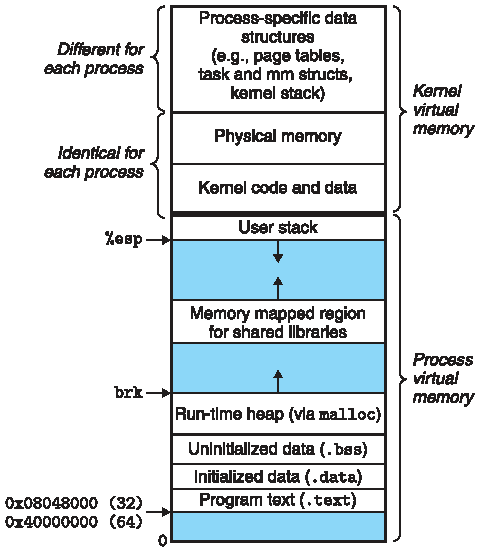
\includegraphics[width=0.5\textwidth]{figures/memory-layout}
	\caption{The memory layout of a Linux process \cite[804]{Bryant2011}}
	\label{fig:memory-layout}
\end{figure}

As \cref{fig:memory-layout} shows, above those memory regions the dynamically growing and shrinking memory regions like the heap, the mapped memory and the stack are located.
Those regions have in common that depending on the program's execution flow, their size changes.
Thus, they need to have free memory around them in order to be able to dynamically grow (marked in blue in \cref{fig:memory-layout}).

The heap contains data which has to be allocated dynamically because the necessary amount of memory is not fixed and has to be determined during runtime.
This includes for example arrays or buffers like the \texttt{input} buffer in \cref{lst:memory-layout}.
As the user input cannot be determined before running the program, the buffer has to be allocated dynamically which happens with a call to \texttt{malloc} in line 11 of the listing.
The contents of the buffer are then stored on the heap.

The stack on the other hand contains data with fixed size.
In the example of \cref{lst:memory-layout}, sizes of variables like \texttt{int max\_len} or \texttt{char *input} are known at compile-time.
Thus, they can be stored on the stack by increasing the stack size by a fixed size when program flow enters the corresponding function.
It has to be noted here that even though the contents of the \texttt{input} buffer are stored in the heap, the pointer to those contents is stored on the stack.

The mapped memory is a region where files from the computers file system are mapped to directly address those files' contents just like other any other memory contents like variables or program instructions.
Such files can be any files accessible by the running program.
The main usage for this feature is to map libraries into memory, for example \gls{glibc} or custom created libraries.

\lstinputlisting[language=C,float=ht,caption={C program containing stack variables as well as heap variables},label={lst:memory-layout}]{code/memory-layout.c}

\section{Stack setup and usage}
\label{sec:stack-setup-and-usage}

As shown in \cref{sec:process-memory}, the stack can contain program data with a size already known at compile time.
It is a data structure behaving according to the \gls{lifo} principle meaning that the data on top of the stack is the data that was put on the stack last and will be removed from the stack first.
When a function is entered, the stack size is increased by the accumulative size of the function's variables by decrementing the stack pointer by this size.
This is also known as ``pushing a stack frame onto the stack'' where \emph{stack frame} refers to the totality of a function's local data.
The stack pointer is stored in the processor register \texttt{esp} (\texttt{x86}/\texttt{i386} architecture) or \texttt{rsp} (\texttt{x86\_64}/\texttt{amd64} architecture) and points to the top of the stack.
On leaving the function, the stack size is decreased by the same amount of memory by incrementing the stack pointer, also known as ``popping a stack frame from the stack''.
This implies that variables declared in a function can only be safely accessed as long as the function is active.
\emph{Active} here means that either control flow is currently inside this function or inside another function called by this function, maybe even recursively.
Otherwise, the memory where those variables reside was already freed by decreasing the stack size and any access to such variables yields nondeterministic behavior.

When a function is called, not only its variables are stored on the stack but also some control flow information like the \gls{rip}.
The \gls{rip} points to the next instruction in the calling function which should be executed after the called function returns.
This is exactly what the \texttt{call} and \texttt{ret} assembly instructions do.
\texttt{call} pushes the address of the next instruction onto the stack and then enters the called function.
In the called function, \texttt{ret} at the end of the function pops the saved address from the stack and continues execution at this address.

Depending on the compiler configuration, there is also often a \gls{sfp} put on the stack which usually lies between the \gls{rip} and the called function's local data on the stack.
Apart from the \texttt{esp/rsp} register, the \texttt{ebp/rbp} register can be used to address stack contents.
At the start of a function, the current \texttt{ebp/rbp} register content is pushed onto the stack as the \gls{sfp} and the \texttt{esp/rsp} content is loaded into \texttt{ebp/rbp}.
Throughout the function, this register's value does not change whereas the \texttt{esp/rsp} value can change through \texttt{push} or \texttt{pop} instructions as the stack pointer should always to the top of the stack.
The static value of the \texttt{ebp/rbp} register thus allows to address a function's stack content by fixed offsets that don't change throughout the function's code and is often referred to as \emph{frame pointer}.
On returning from a function, the \gls{sfp} is loaded into \texttt{ebp/rbp} to allow the caller function to use its static offsets into its own stack frame again when continuing its execution.

Thus, the stack not only contains data but also important control flow information.

\section{Stack Buffer Overflows}
\label{sec:stack-buffer-overflows}

This mixture of data and control flow information is exactly where problems arise.

Under the assumption that a function exists somewhere in a program as shown in \cref{lst:vulnerable-function}, the stack layout of such a function may look as shown in \cref{fig:stack-layout-without-data}.
After the \gls{rip}, the compiler by default usually positions the \gls{sfp} and the local variables in the order they were declared%
	\footnote{
		The layout as shown in \cref{fig:stack-layout} should just be seen as an example, as it can differ depending on compiler behavior or processor architecture (here: 32 bit architecture with stack alignment on 4 bytes, function arguments passed on the stack).
	}%
.

\begin{lstlisting}[language=C,float=ht,caption={C function with buffer overflow vulnerability}, label={lst:vulnerable-function}]
void copy(char *bar) {
    char c[12];
    strcpy(c, bar);
}
\end{lstlisting}

A stack buffer overflow vulnerability here lies in the call to \texttt{strcpy} in line 6.
This function copies a string from the memory location where \texttt{bar} points to to the memory location where \texttt{c} points to.
However, it copies data until it encounters a \texttt{0x00} byte which marks the end of the string, regardless of whether the destination can take all the copied data.

If the string to copy is strictly less than 12 bytes, no problem occurs as the buffer can hold the string (11 bytes at maximum) and the string terminating \texttt{0x00} byte as shown in \cref{fig:stack-layout-no-overflow}.

If the string to copy is 12 bytes or more, a buffer overflow occurs as shown in \cref{fig:stack-layout-overflow}.
This means that the \texttt{strcpy} function copies 12 bytes or more of data to the buffer \texttt{c} even though it cannot hold more than 12 bytes.
Including the terminating \texttt{0x00} byte, this string copy operation thus overwrites data residing on the stack after the destination buffer.

\begin{figure}[htb]
	\centering
	\begin{subfigure}[t]{0.3\textwidth}
		\centering
		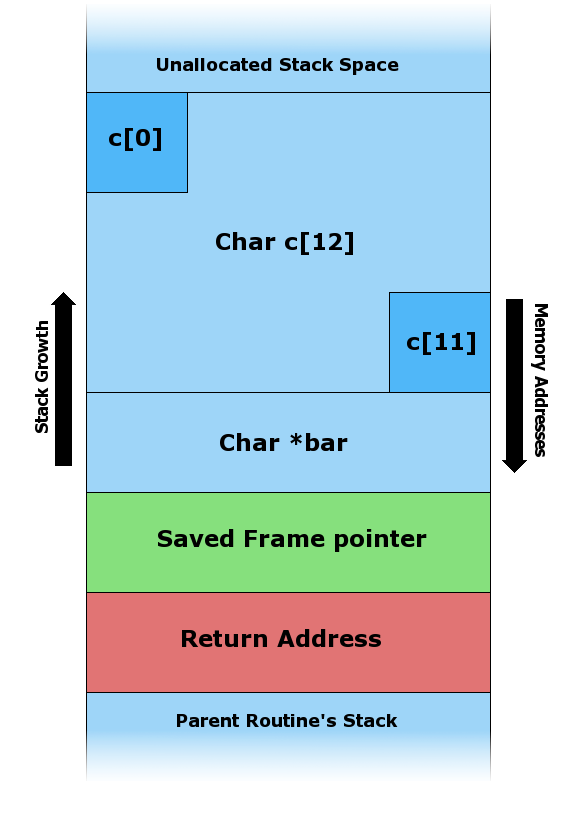
\includegraphics[height=0.25\textheight]{figures/Stack_Overflow_2}
		\caption{Stack layout with control flow information and local data \cite{Lynn2007}}
		\label{fig:stack-layout-without-data}
	\end{subfigure}
	\hfill
	\begin{subfigure}[t]{0.3\textwidth}
		\centering
		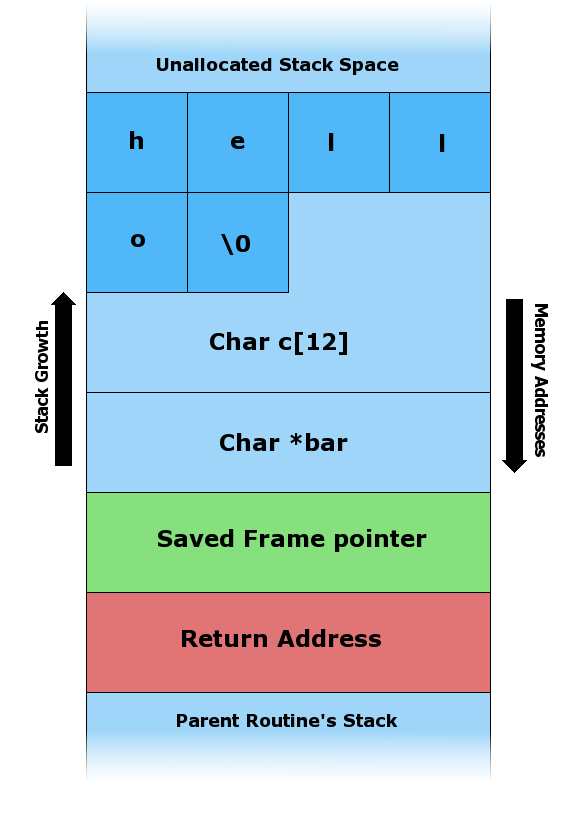
\includegraphics[height=0.25\textheight]{figures/Stack_Overflow_3}
		\caption{Stack contents after copying data to the \texttt{char} array without overflowing it \cite{Lynn2007a}}
		\label{fig:stack-layout-no-overflow}
	\end{subfigure}
	\hfill
	\begin{subfigure}[t]{0.3\textwidth}
		\centering
		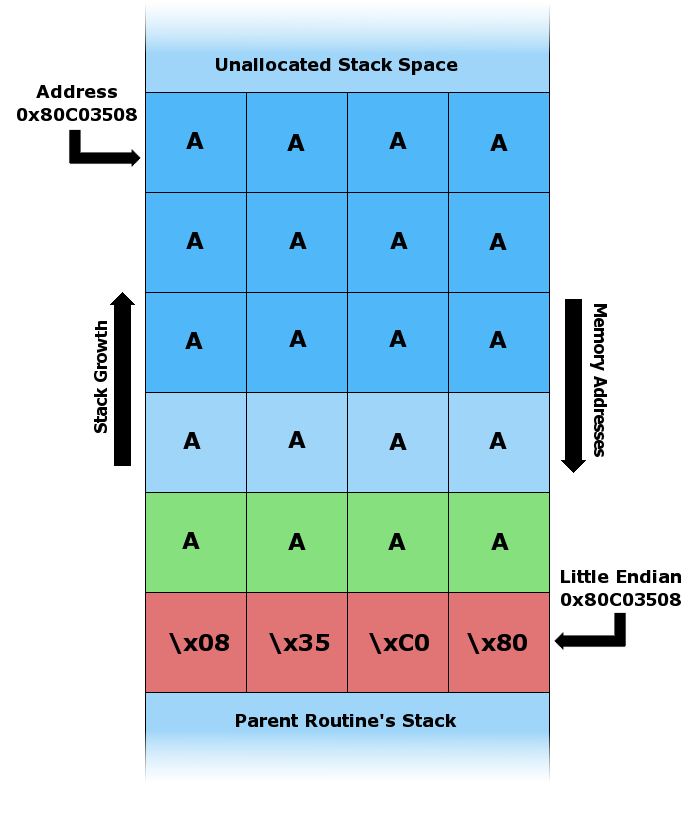
\includegraphics[height=0.25\textheight]{figures/Stack_Overflow_4}
		\caption{Stack contents after copying data to the \texttt{char} array and overflowing it \cite{Lynn2007b}}
		\label{fig:stack-layout-overflow}
	\end{subfigure}
	\caption{Stack layout of a function with two local variables: a 12 byte buffer (\texttt{char c[12]}) and a pointer (\texttt{char *bar})}
	\label{fig:stack-layout}
\end{figure}
\todo{If enough time, edit all graphics to represent 64 bit stacks}

If an attacker can control the data which is copied onto the stack, they%
	\footnote{In this paper, the gender-neutral singular pronoun ``they'' and pronouns derived from it are used instead of singular ``he'', ``she'' or pronouns derived from those if no specific gender is provided for a person.}
	\todo{Check if this is the first occurrence, otherwise move footnote to the first one}
can carefully craft an input string so that they can overwrite the \gls{sfp} or \gls{rip} with attacker-controlled data and thus control where the program tries to look for function-local data (overwritten \gls{sfp}) or to continue execution (overwritten \gls{rip}) after it returns from the current function.
A stack buffer overflow always occurs if a buffer just like \texttt{c} in \cref{lst:vulnerable-function} is filled with more data than it can hold.
This does not necessarily mean that the \gls{sfp} or \gls{rip} is overwritten by a stack buffer overflow, but in most cases this is the goal of an attacker in order to divert control flow in the program's execution or manipulate a function's data.

How an attacker can divert control flow or manipulate data and what implications come with this possibility is explained in \cref{chp:attack-vectors}.


\chapter{Current defense mechanisms}
\label{chp:current-defense-mechanisms}

This chapter provides information about defense mechanisms trying to mitigate stack buffer overflow attacks as they are currently employed by the Linux kernel or the compiler.
This refers to software versions as described in \cref{sec:system-model}.

\Cref{chp:attack-vectors} then describes the actual attack possibilities that arise from a stack buffer overflow vulnerability and how such attack vectors can be rendered unusable or at least inefficient and hard to exploit.

Additionally, some of the attacks described in \cref{chp:attack-vectors} can also be used to bypass some of the mitigation measures described in \hyperref[chp:current-defense-mechanisms]{this \namecref{chp:current-defense-mechanisms}}.
Therefore, \cref{chp:defense-mechanism-improvements} provides different approaches on how to improve the defense mechanisms in order to prevent even more attacks.

\section{Compiler-based measures}
\label{sec:compiler-based-measures}

\subsection{The \texttt{\_FORTIFY\_SOURCE} macro}
\label{subsec:fortify-source}

Support for the \texttt{\_FORTIFY\_SOURCE} macro was added to \gls{gcc} in \citedate{Jelinek2004} and is available since \gls{gcc} version 4.0 \cite{Sharma2014}.
The possible values for this macro are 0, 1 and 2 with 0 meaning that it has no effect and 2 meaning that all measures that are implied by this macro are active.

The effect of this macro is that the compiler checks at compile time as well as at run time whether a destination buffer is overflown by functions such as \texttt{strcpy}, \texttt{strncat}, \texttt{memcpy}, and so forth%
	\footnote{Supported functions according to \cite{Kerrisk2020,Sharma2014}: \texttt{memcpy, mempcpy, memmove, memset, strcpy, stpcpy, strncpy, strcat, strncat, sprintf, vsprintf, snprintf, vsnprintf, gets}}%
.
In order to achieve this, the compiler checks at compile time whether the destination is big enough to hold the source's contents.
This is done by comparing function arguments (e.g. the number of bytes to set in \texttt{memset}) or array sizes, if the source and destination arrays have fixed sizes.
If the compiler detects an overflow, it issues a warning \cite{Jelinek2004,Kerrisk2020,Sharma2014,Sidhpurwala2018}.

For dynamic sized operands where the compiler cannot determine whether the destination operand will be overflown, the function calls are replaced with wrapper functions that check the operands' sizes.
For example, \texttt{strcpy} is replaced with \texttt{\_\_strcpy\_chk}.
If the check fails, the program execution is aborted with an error message \cite{Kerrisk2020,Sharma2014}.

The \texttt{\_FORTITY\_SOURCE} macro can either be manually set to a value higher than 0 or is automatically activated when compiler optimizations are enabled, for example by passing the \texttt{-O3} flag to \gls{gcc} \cite{Kerrisk2020,Sharma2014,Sidhpurwala2018}.
\todo{Include example? Not sure}

\citename{Jelinek2004} states in the announcement of the original implementation of this feature that the run time overhead of the checks is very small and that the compiler automatically omits the checks if it can prove at compile time that no overflow can occur \cite{Jelinek2004}.


\begin{itemize}
	\item{
		\texttt{ebp} mostly not used as frame base pointer register but as standard register when optimizations are enabled $\Rightarrow$ other stack layout
	}
\end{itemize}

\section{\glsentrylong{dep} (\glsentryshort{dep})}
\label{sec:data-execution-prevention}

\begin{itemize}
	\item{NX bit}
	\item{W $ \oplus $ X page permissions}
\end{itemize}

\section{Function Pointer Protection}
\label{sec:function-pointer-protection}

\section{\glsentrylong{aslr} (\glsentryshort{aslr})}
\label{sec:address-space-layout-randomization}

\begin{itemize}
	\item{Randomized on program startup}
	\item{Clone-probing attacks: no new randomization on \texttt{fork}}
\end{itemize}

\section{Stack canaries}
\label{sec:stack-canaries}

\begin{itemize}
	\item{Random canary created on program startup}
	\item{Same canary for all functions $\Rightarrow$ canary disclosure in one function makes all other functions vulnerable}
	\item{Clone-probing attacks: no new randomization on \texttt{fork}}
\end{itemize}

\section{Control Flow Integrity}
\label{sec:cfi}

\begin{itemize}
	\item{Intel CET $\Rightarrow$ shadow stack, branch validation}
\end{itemize}
\chapter{Attack vectors}
\label{chp:attack-vectors}

In this chapter, we describe several methods to gain control over a program vulnerable to stack buffer overflow attacks.
In each of the sections, it is assumed that none of the measures from \cref{chp:current-defense-mechanisms} are enabled or active unless otherwise stated.

\todo{
 Differentiate between RIP and SFP overwriting? 
 If yes, in sections if applicable or in own section?
 What about overwriting data in general?
 Maybe own section at the end? Or somewhere in the middle?
%\section{Overwriting \glsentryshort{rip} and \glsentryshort{sfp}}
}

\section{Code injection}
\label{sec:code-injection}

\subsection{Operating principle}
\label{subsec:ci-operating-principle}

Code injection is the simplest attack vector for stack buffer overflows.
As described in \cref{sec:stack-buffer-overflows}, an attacker might try to overwrite the \gls{rip}.
If this is possible, an attacker can divert control flow to any location he wants.

At such locations, the attacker can place so-called \emph{shellcode} before overflowing the vulnerable buffer.
Shellcode is the binary representation of assembly instructions compiled to the corresponding \glspl{opcode}.
Such code can be directly executed by the processor without the need of compilation (high-level programming languages like C) or translating assembly instructions with an assembler.
Shellcode can be created by compiling the desired code or assembling the desired assembly instructions into an executable file.
The executable binary shellcode can then be extracted from the resulting binary file%
	\footnote{Public databases like \href{https://www.exploit-db.com/shellcodes}{exploit-db.com} already provide lots of pre-compiled shellcode suitable for different architectures and \glspl{os}.}%
.
The name \emph{shellcode} is derived from the general attacker's goal to spawn a shell and thus execute arbitrary commands.
However, shellcode can contain any instructions and does not necessarily have to spawn a shell on the attacked system directly.

\subsubsection{Code injection into the vulnerable buffer}
\label{subsubsec:ci-into-vuln-buffer}

One possibility for an attacker to execute shellcode is to place the shellcode into the buffer which is overflown before the \gls{rip} value, as they control the buffer's contents.
The return address then has to be overwritten with the address of the buffer on the stack.
If the right address is used, the program does not return to the caller function as intended but to the position on the stack where the overwritten buffer is located.
The processor then tries to decode the data on the stack as processor instructions and thus executes the shellcode stored in the buffer.

Such an attack is very hard to achieve correctly, as the return address written onto the stack has to match the buffer's address exactly.
An offset of the return address to the buffer's address of a single byte can already render the shellcode unusable, as the instructions are decoded incorrectly by the processor.
Thus, a common technique to improve the reliability of such an exploit is to include a so-called \emph{\gls{nop} sled} into the user-controlled input which is used to overflow the vulnerable buffer on the stack.
A \gls{nop} sled consists of binary encoded \acrshort{nop} assembly instructions (byte \texttt{0x90} on \texttt{x86/x86\_64}).
This instruction tells the processor to do nothing during the cycle where this instruction is executed.
If a lot of such instructions are placed in front of the shellcode into the buffer, the return address does not necessarily have to point exactly to the start of the buffer or the start of the shellcode but it is sufficient to point the return address to a location somewhere in the \acrshort{nop} sled.
When returning into the \acrshort{nop} sled, the processor then executes several \gls{nop} instructions and progresses on the stack until it reaches the shellcode.

It is also possible to place the \acrshort{nop} sled after the shellcode on the stack instead of in front of the shellcode.
If the length of the shellcode and the \acrshort{nop} sled is known, a relative jump can be added to the end of the \acrshort{nop} sled with the negative offset for the relative jump being the combined length of the shellcode and the \acrshort{nop} sled.
As shown in \cref{fig:stack-overflow-nop-sled}, such a \acrshort{nop} sled can even extend over the overwritten return address with the help of a second relative jump in order to bypass size restrictions given by the size of the buffer.

\begin{figure}[htb]
	\centering
	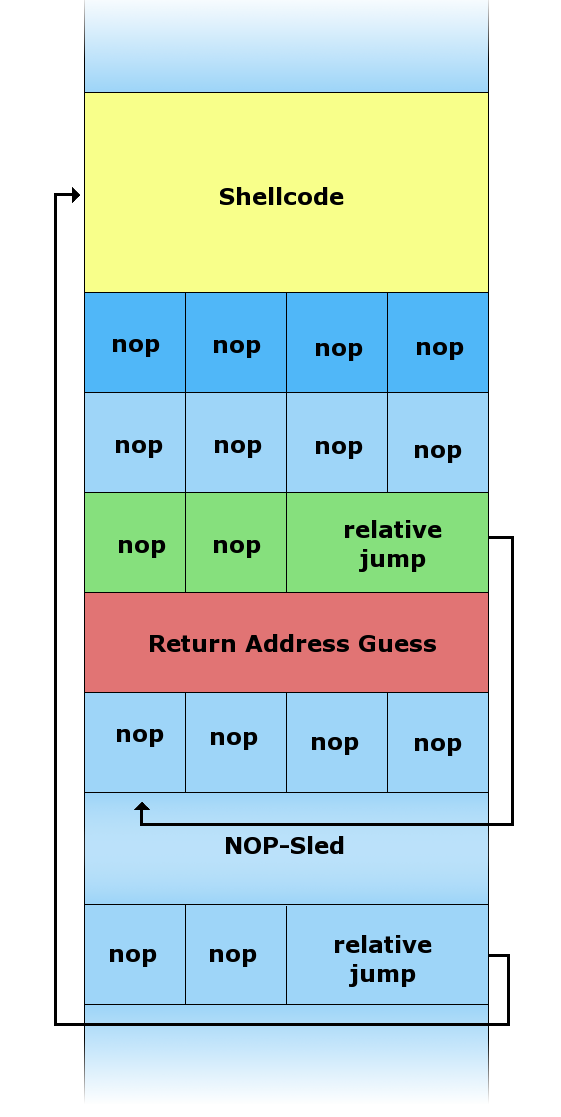
\includegraphics[width=0.3\textwidth]{figures/NopSled}
	\caption{Stack layout after a stack buffer overflow with shellcode and \acrshort{nop} sled \cite{Lynn2007c} (cf. \cref{fig:stack-layout})}
	\label{fig:stack-overflow-nop-sled}
\end{figure}

In general, a long \acrshort{nop} sled is desired by an attacker, as it becomes easier to guess an address inside of the \acrshort{nop} sled \cite{AlephOne1996}.

\subsubsection{Code injection via environment variables}
\label{subsubsec:ci-via-env-variable}

If it is desired to have a contiguous block of shellcode with maybe a \acrshort{nop} sled in front of it without the necessity of relative jumps, it might be a problem to have the exploit code fit into the vulnerable buffer before the overwritten return address, as the buffer might be too small to store the whole input.
In such cases, the actual exploit code (\acrshort{nop} sled and shellcode) can be put into an environment variable on the system which is being attacked if the attacker has the necessary access to the system to set environment variables.
There are slight offsets depending on the contents of other environment variables, but an environment variable generally can be found at the same address in each started process, as environment variables are loaded at the bottom of the stack \cite[731\psq]{Bryant2011}.
This allows to retrieve the location at which an environment variable will be located in the attacked process with the help of a second program (cf. \cref{lst:getenvaddress}).

Thus, it is possible to point the return address into an environment variable instead of the overflown buffer.
If the return address successfully points either directly to the shellcode or into the \acrshort{nop} sled inside the environment variable, the shellcode is executed exactly as in the previous case where it was put into the user-controlled overflown buffer.

A restriction of this approach is that environment variables are only mapped into the processes address space when the process is started.
Thus, shellcode cannot be injected into already running programs with the help of environment variables but only into programs started after setting the environment variable.

\subsubsection{Code injection into global variables}
\label{subsubsec:ci-via-globals}

If the shellcode is put into an environment variable, it is pretty easy to locate in memory as described above.
If this is not possible because an attacker wants to target an already active process, the shellcode has to be written onto the stack.
The difficulty of this approach is to find suitable addresses to point the \gls{rip} to when overflowing a vulnerable buffer, as stack addresses are highly volatile depending on the depth of the call stack and the functions' local variables.

If there is the possibility to place data in a global buffer before overflowing the local buffer as shown in \cref{lst:local-global-buffer}, an attacker can also put the shellcode into the global buffer and overwrite the \gls{rip} by overflowing the local buffer so that it points into the global buffer.
This greatly eases finding the target address in comparison to stack addresses, as global variables are located in the \texttt{.bss} (uninitialized global variables) or \texttt{.data} (initialized global variables) sections in an \gls{elf} executable and thus are loaded at specific memory locations as seen in \cref{lst:local-global-buffer-disassembly,fig:memory-layout}.
In the given example, the global buffer is always located at the address \texttt{0x0000000000404080}.

\lstinputlisting[language=C,float=ht,caption={C program reading data from \texttt{\acrshort{stdin}} into a global and a local buffer},label={lst:local-global-buffer}]{code/local-global-buffer.c}

\begin{lstlisting}[language=bash,float=ht,caption={Disassembly excerpt of the 64 bit binary compiled from the code in \cref{lst:local-global-buffer} with \texttt{gcc -o local-global-buffer local-global-buffer.c -no-pie}, retrieved with \texttt{objdump -D local-global-buffer}}, label={lst:local-global-buffer-disassembly}]
        ...

Disassembly of section .bss:

0000000000404060 <completed.7393>:
...

0000000000404080 <global_buffer>:
...
\end{lstlisting}

\subsubsection{Code injection into arbitrary buffers}
\label{subsubsec:ci-into-arbitrary-buffer}

Shellcode can also be read into any local buffer on the stack that is user-controlled before overflowing the vulnerable buffer.
However, as already mentioned \hyperref[subsubsec:ci-via-globals]{above}, it can be difficult to locate such a buffer on the stack even when using a \acrshort{nop} sled.

\subsection{Difficulties and countermeasures}
\label{subsec:ci-countermeasures}

Over the last 24 years since \citeauthor{AlephOne1996}'s article \citetitle{AlephOne1996} was published, several changes in processor architecture, such as the transition from 32 bit \texttt{x86} to 64 bit \texttt{x86\_64}, as well as lots of newly introduced mitigation techniques made it difficult or even impossible to inject code into a program's address space and execute such code.

\subsubsection{64 bit addressing}
\label{subsubsec:ci-64bit-addressing}

With the transition from \texttt{x86} to \texttt{x86\_64}, the addresses changed from a length of 32 bits / 4 bytes to 64 bits / 8 bytes.
However, the Linux kernel with the default 4-level page tables only uses 47 of the address bits for userspace virtual memory addresses and sets the upper 17 bits to zero.
With 5-level page tables, 56 bits are utilized and the upper 8 bits are set to zero \cite{Kernel2020}.

This fact implies that there is always at least one \texttt{0x00} byte in an address.
As such a \texttt{0x00} byte also marks the end of a string, an attacker might not be able to write past such a byte if the overflow occurs in a string operation function, such as \texttt{strcpy} or \texttt{gets}.
As the aforementioned processor architectures use little-endian byte addressing%
	\footnote{Least significant byte first in comparison to big-endian addressing with most significant byte first}%
, the \texttt{0x00} bytes come last and thus probably don't impose any problems when overwriting the return address, as the upper bytes are already set to \texttt{0x00} because of the original return address also being a userspace virtual memory address. 
However, usually a \gls{sfp} also has to be overwritten before even reaching the \gls{rip} (cf. \cref{fig:stack-layout}).
Because of this pointer also being a userspace virtual memory address, it also has the upper bytes set to \texttt{0x00} and can cause problems when overflowing a buffer with string based functions.

In an example as in \cref{lst:local-global-buffer}, this problem does not occur because \texttt{read} as a binary input function is used instead of string input functions.

\subsubsection{\glsentrylong{dep} (\glsentryshort{dep})}
\label{subsubsec:ci-data-execution-prevention}

Seeing that the \gls{nx} bit is used by the Linux kernel by default (cf. \cref{sec:executable-space-protection}), \gls{dep} features prevent stack contents from being executable by default.
For the stack being marked as executable, the \texttt{-z execstack} command line parameter has to be passed to \gls{gcc} explicitly.

Thus, it is not possible to make use of code injection into a process's address space on modern \glspl{os}, as the injected code is located on memory pages marked as non-executable.
This not only includes a function's local stack memory but also the memory areas where environment variables are located as well as memory regions used for storing global variables.

\subsubsection{\glsentrylong{aslr} (\glsentryshort{aslr})}
\label{subsubsec:ci-aslr}

Even if user-writable memory regions are marked as executable, for example because a \gls{jit} compiler needs to store generated code, \gls{aslr} can make it extraordinarily harder for an attacker to overwrite code pointers such as the \gls{rip} or function pointers with addresses pointing to valid memory areas and especially pointing to the user-generated shellcode or into a \gls{nop} sled.

However, \gls{aslr} has several weaknesses which are further described in \cref{chp:defense-mechanism-improvements} and where bypass approaches are presented in following sections.
\todo{Make reference more concrete than just referring to a whole chapter}

In general, the combination of \gls{dep} and \gls{aslr} provides a strong defense against code injection stack buffer overflow attacks.

\section{Returning into executable code}
\label{sec:returning-into-executable-code}

\subsection{Return-to-libc (\glsentryshort{ret2libc})}
\label{subsec:ret2libc}

\subsection{\glsentrylong{rop} (\glsentryshort{rop})}
\label{subsec:rop}

\subsection{\glsentrylong{jop} (\glsentryshort{jop})}
\label{subsec:jop}

\subsection{\glsentrylong{cop} (\glsentryshort{cop})}
\label{subsec:cop}

% Depending on time left!
\chapter{OS assessment}
\label{chp:os-assessment}

\todo[inline]{Probably not enough time left}

\begin{itemize}
	\item{If enough time left at the end}
	\item{Scan different Linux distributions' /bin directory for insecure applications}
	\item{Example: \texttt{snapctl} on Ubuntu 20.04: no stack canaries, no position independent executable, no \gls{relro}}
\end{itemize}

%% Contains placeholder stuff

\chapter{Einleitung}
\label{chp:Einleitung}
Lorem ipsum dolor sit amet, consectetuer adipiscing elit, sed diam nonummy nibh euismod tincidunt ut laoreet dolore magna aliquam erat volutpat. Ut wisi enim ad minim veniam, quis nostrud exerci tation ullamcorper suscipit lobortis nisl ut aliquip ex ea commodo consequat. \cite{Konak2006,Sailer2013}

Lorem ipsum dolor sit amet, consectetuer adipiscing elit, sed diam nonummy nibh euismod tincidunt ut laoreet dolore magna aliquam erat volutpat. Ut wisi enim ad minim veniam, quis nostrud exerci tation ullamcorper suscipit lobortis nisl ut aliquip ex ea commodo consequat.
 
 
 \chapter{Hauptteil}
 \label{sec:Hauptteil}
 
 Abbildungen k\"{o}nnen im Unterverzeichnis \texttt{figures} abgelegt werden.
 Eingebunden werden Sie mit dem Befehl \texttt{\textbackslash includegraphics} innerhalb
 einer \texttt{figure}-Umgebung:
 \begin{figure}[htb]
 	\centering
 	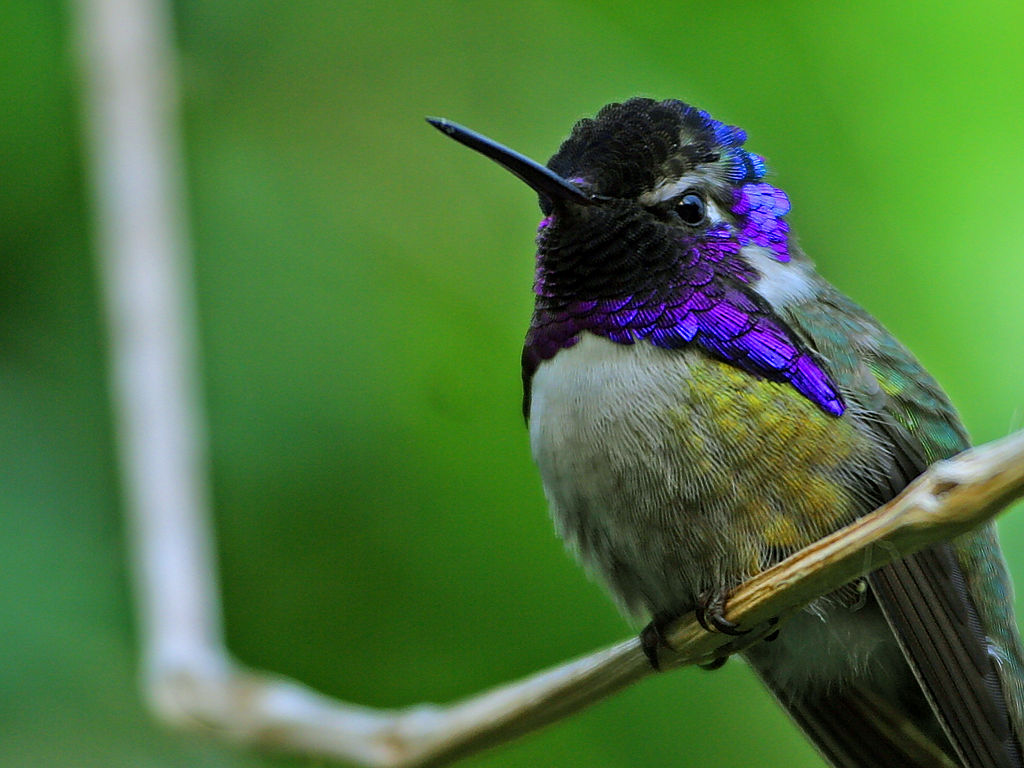
\includegraphics[width=0.8\textwidth]{figures/Hummingbird.jpg}
 	\caption{Eine Veilchenkopfelfe (auch Costakolibri genannt, vom lateinischen Calypte costae), die zur Familie der Kolibris geh\"{o}rt \cite{Kolibri}}
 	\label{fig:kolibri}
 \end{figure}
 
 \section{Erste Zwischen\"{u}berschrift}
 \label{sec:ErsteZwischenueberschrift}
 Die Arbeit kann auch Tabellen im \texttt{table}-Environment enthalten:
 \begin{table}[ht]
 	\centering
 	\caption{Entfernungstabelle S\"{u}ddeutschland, vgl. \cite{entfernungstabelle}}
 	\begin{tabular}{c r r r}
 		\toprule
 		& Augsburg & M\"{u}nchen & Stuttgart \\
 		\midrule
 		Augsburg  & -        & 61      & 149       \\
 		M\"{u}nchen   & 61       & -       & 210       \\
 		Stuttgart & 149      & 210     & -         \\
 		\bottomrule
 	\end{tabular}
 	\label{tab:entfernungen}
 \end{table}
 
 \subsection{Erste Unter\"{u}berschrift}
 \label{sec:ErsteUnterueberschrift}
 
 Das \texttt{listings}-Paket erlaubt es, Quellcode mit Syntax-Highlighting einzubinden:
 
 \begin{lstlisting}[language=Python,float=ht,caption={Python-Programm zur Berechnung der Fakult\"{a}tsfunktion}]
 def fact(n):
 """Return the n-th factorial number"""
 if n == 0:
 return 1
 else:
 return n * fact(n-1)
 
 # Test output
 print fact(10)
 print "Done"
 \end{lstlisting}
 \label{lst:factorial}  
 
 \section{Zweite Zwischen\"{u}berschrift}
 \label{sec:ZweiteZwischenueberschrift}
 
 TEXT
 
 \chapter{Schluss}
 \label{chp:Schluss}
 
 TEXT
 
 %%% Local Variables:
 %%% mode: latex
 %%% TeX-master: "../Abschlussarbeit"
 %%% End:
 

% Anhang
\appendix

\chapter{Beweis von P = NP}

Lorem ipsum dolor sit amet, consectetuer adipiscing elit, sed diam nonummy nibh euismod tincidunt ut laoreet dolore magna aliquam erat volutpat. Ut wisi enim ad minim veniam, quis nostrud exerci tation ullamcorper suscipit lobortis nisl ut aliquip ex ea commodo consequat.

Lorem ipsum dolor sit amet, consectetuer adipiscing elit, sed diam nonummy nibh euismod tincidunt ut laoreet dolore magna aliquam erat volutpat. Ut wisi enim ad minim veniam, quis nostrud exerci tation ullamcorper suscipit lobortis nisl ut aliquip ex ea commodo consequat.

%%% Local Variables:
%%% mode: latex
%%% TeX-master: "Report"
%%% End:


% Literaturverzeichnis
\begin{otherlanguage}{british}
	\printbibliography[heading=bibintoc]
\end{otherlanguage}

% Eidesstattliche Erklärung
\clearpage
\section*{\GetTranslation{honesty@title}}
\GetTranslation{honesty@body}

\vspace{2em}
\makeatletter
Orsay, \@date
\par\vspace{1.5cm}
(\@author)
\makeatother

%%% Local Variables:
%%% mode: latex
%%% TeX-master: "Report"
%%% End:


\end{document}

%%% Local Variables:
%%% mode: latex
%%% TeX-master: t
%%% End:
